The following sections describe the system design of the Android application. All functionality of the system components are described in this section. Worth noting is that the figures referred to in this section can be found further down in the document.

\subsection{System overview}
	The Android application is divided into eight \emph{packages}. These packages are \verb!default!, \verb!com!, \verb!login!, \verb!model!, \verb!processing!, \verb!search!, \verb!search_result! and \verb!selected_files!.
	All packages (except for \verb!com! and \verb!model!) contains one or several pairs of activities and fragments. An \verb!Activity! is a single, focused thing the user can do. A \verb!Fragment! is an object that helps to modularize the code and brings more sophisticated user 	interfaces.

	\begin{figure}[h]
		\centering
		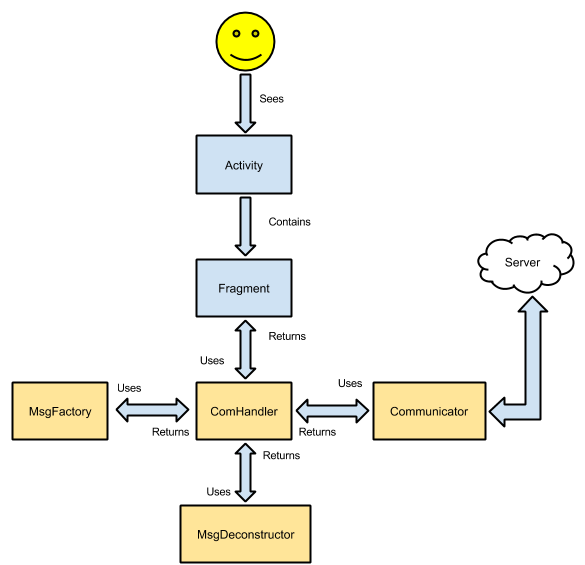
\includegraphics[width=1\textwidth]{and_system_overview.png}
		\caption{\label{fig:and_system_overview}A generalization of how the Android application works.}
	\end{figure}

	The user will interact with an activity that holds a fragment. The fragment (which contains some logic) will tell the class \verb!ComHandler! what action that should be performed. The \verb!ComHandler! will construct a message by using \verb!MsgFactory!. The message is then passed on to \verb!Communicator! which sends the message to the server with REST. The \verb!Communicator! returns the response to the \verb!ComHandler! that parses it by using the class \verb!MsgDeconstructor! and then returns it to the fragment. Hopefully, \refer{fig:and_system_overview} will bring some clarity.
	
\subsection{Package overview}
	The \verb!default! package only contains one class, \verb!SingleFragmentActivity!. This class is the base of every screen in the application. It is responsible for the navigation in the application and to inflate the correct \verb!ActionBar!. All other activities extends this 	class.

	The \verb!com! package is responsible for communication with the server. It also contains classes and methods for construction and deconstruction of JSON.

	The \verb!login! package contains the GUI and controller for the login screen. It also enables the user to select, add, edit and delete server URLs.
	
	The \verb!model! package holds information about experiments, annotations, files etc. found on the server.
	
	The \verb!processing! package is responsible for displaying processing parameters etc. for when the user wants to process a certain file.
	
	The \verb!search! package handles searches by either selecting annotations, or by manually typing in PubMed style.
	
	The \verb!search_result! package handles the results of the search by displaying the experiments found. When an experiment is selected, the files associated with the experiment is displayed.
	
	The \verb!selected_files! handles all the files that has been selected. They are sorted into raw, profile and region. The raw files can be selected for processing from here.

\subsection{Class description}
\begin{figure}[h]
\begin{tabularx}{\textwidth}{|l|X|}
\multicolumn{2}{l}{\strongTerm{Fragment classes}} \\
\hline
\term{LoginFragment} &
LoginFragment is the first view to be visualized when the application is started. It allows the user to connect to a server by specifying username and password. The static class ComHandler is used to send and validate the login request. If the username and password are incorrect the user will be informed through an android toast explaining what happened. Likewise if the server cannot be reached.
A successful login will start the SearchListFragment.
\\ \hline
\term{SettingsFragment} &
SewttingsFragment is used for selecting which server to use. There is also choices for adding, deleting and editing server locations.
\\ \hline
\term{SearchListFragment}\label{sec:and_class_search} &
SearchListFragment is the search-view for the \appName\ app, the annotations that can be chosen are downloaded from the server and they are, as such, dynamic.
\\ \hline
\term{SearchPubmedFragment} &
SearchPubmedFragment is a fragment that handles the search if the user want to manipulate it with the PubMed style of input. When started the current search from the searchFragment is converted and displayed for the user, who can continue using the choosen search values in a PubMed style.
\\ \hline
\term{SearchSettingsFragment} &
SearchSettingsFragment handles settings for which annotations are displayed in the search result. Available annotations is shown in a ListView and there is option to select annotations and save into internal storage. There is an option to set default settings which will show first two available annotations together with experiment name and who the experiment is created by. Settings for using available settings or using default settings is stored in a file in internal storage.
\\ \hline
\term{ExperimentListFragment} &
ExperimentListFragment handles the displaying of search results to the user. The fragment includes a ListView with an ArrayAdapter set to it. An OnItemClickListener is used to detect when the user is selecting an item in the list and is currently starting FileListActivity when a list item is selected. This fragment receives a HashMap with search values from SearchListFragment and when activity is starting an ASyncTask is started to send and receive search results from the server through the ComHandler class. When an experiment is selected from the list the file names belonging to that experiment is sent to FileListFragment that will display the file information.
\\ \hline
\end{tabularx}
\end{figure}
\begin{figure}[h]
\begin{tabularx}{\textwidth}{|l|X|}
\multicolumn{2}{l}{\strongTerm{Fragment classes}} \\
\hline
\term{FileListFragment}\label{sec:and_class_filelist} &
FileListFragment displays all files associated with a chosen experiment. The fragment is using three ListViews, one for each data type. The data types that are available are: raw, region and profile. Each list element will show the name of the data file and have a checkbox connected to it. A custom ArrayAdapter is used to handle checkbox interaction and displaying information to the user. There is option to select multiple files in the view by checking several checkboxes. The file names displayed are the ones currently available from the server for each available experiment.
\\ \hline
\term{SelectedFilesFragment} &
SelectedFilesFragment gives the user an overview of all files added to the selected files. The view contains a TabHost which in turn consists of a number of fragments. The selectedFilesFragment lets the user explore the tabs by either swipe or by simply pressing the tab the user wishes to see. The tabs consists of the following fragments; RawFragment, ProfileFragment, RegionFragment.
\\ \hline
\term{RawFragment}\label{sec:and_class_rawfragment} &
RawFragment keeps track of all raw-files added to the selected files. When this fragment is first created it collects all saved raw files of the type raw from the DataStorage and initializes a listview, visualizing the objects.
\\ \hline
\term{ProfileFragment}\label{sec:and_class_profilefragment} &
ProfileFragment keeps track of all profile-files added to the selected files. When this fragment is first created it collects all saved files of the type profile from the DataStorage and initializes a listview, visualizing the objects.
\\ \hline
\term{RegionFragment}\label{sec:and_class_regionfragment} &
RegionFragment keeps track of all region-files added to the selected files. When this fragment is first created it collects all saved files of the type region from the DataStorage and initializes a listview, visualizing the objects.
\\ \hline
\end{tabularx}
\end{figure}
\begin{figure}[h]
\begin{tabularx}{\textwidth}{|l|X|}
\multicolumn{2}{l}{\strongTerm{Fragment classes}} \\
\hline
\term{ConverterFragment} &
ConverterFragment displays to the user all the different parameters the conversion can have and what is expected of them. The different inputfields are connected together, so that the user has to fill them out in the right order to be able to get access to the next field. There are some exceptions to that manner, the first two parameters Bowtie and Genome-release has to be used to start a conversion. After that the following fields has to be filled out to gain access to the next inputfield, the last two fields are also an exception to that as they are linked together to form the parameters for the ratio-calculation. When created the fragment calls the server in an async-task and retreives information about the different genome-releases that is to be found on the server, a spinner with the choices are setup when downloaded. The inputfields are collected when the user press the convert button, by checking which fields/toggleButtons that are enabled. When collected the parameters are sent to the server in another async-task, when the conversions are started and confirmed by the server the ProcessFragment is started up.
\\ \hline
\term{ProcessFragment} &
ProcessFragment is a fragment that presents the user with information about the status of the different conversions that is currently under progress on the server. When created, the fragment will start an async-task and retreive current conversion status from the server. The information is visualized in a listview.
\\ \hline
\end{tabularx}
\end{figure}
\begin{figure}[h]
\begin{tabularx}{\textwidth}{|l|X|}
\multicolumn{2}{l}{\strongTerm{Model classes}} \\ \hline
\term{ComHandler}\label{sec:and_class_comhandler} &
ComHandler is a static object that is called by the fragments in the view to gain access to the models different functions. At this stage the ComHandler can be used to login, search for files and to request raw to profile conversions, although the latter is not yet integrated. The url that ComHandler tries to communicate with can be changed with a public method which makes it possible to implement a way for the user to change server.
\\ \hline
\term{Communicator} &
Communicator is used to manage the sending and receiving of messages between the server and the application using a http connection.
\\ \hline
\term{MsgFactory} &
MsgFactory creates the JSON messages that can be sent to the server.
\\ \hline
\term{MessageDeconstructor} &
MessageDeconstructor interprets JSON messages and returns appropriate information.
\\ \hline
\term{GenomizerHttpPackage} &
GenomizerHttpPackage stores the body and status code of an http-response.
\\ \hline
\term{GeneFile} &
GeneFile is used to store and transfer the information of a genome file.
\\ \hline
\term{Annotation} &
Annotation is used to store and transfer one or several annotations and their value.
\\ \hline
\term{Experiment} &
Experiment is used to store and transfer information about an experiment.
\\ \hline
\term{ProcessingParameters} &
ProcessingParameters is used to simplify the transfer of parameters in a processing request.
\\ \hline
\term{DataStorage} &
DataStorage is used to save lists of GeneFile objects on the device locally. DataStorage is a static class, which makes it possiblr to access the saved data anywhere in the application. This simplify the transfer of files between activities.
\\ \hline
\term{GenomeRelease} &
The GenomeRelease class is used to store information about a genomerelease.
\\ \hline
\term{ProcessStatus} &
ProcessStatus is used to store information about the status of a process.
\\ \hline
\term{Genomizer} &
The purpose of Genomizer is to make it possible to create and visualize toasts anywhere in the application. Genomizer is a static class that extends Application.
\\ \hline
\end{tabularx}
\end{figure}
